% Compilar a .pdf con LaTeX (pdflatex)
% Es necesario instalar Beamer (paquete latex-beamer en Debian)
%


\documentclass{beamer}
\usetheme{Warsaw}
\beamertemplatenavigationsymbolsempty
\setbeamertemplate{headline}{}
\useoutertheme{infolines}
\usepackage[utf8]{inputenc}
\usepackage{graphics}
\usepackage{amssymb} % Simbolos matematicos
\usepackage{multicol}

%% Metadatos del PDF.
\hypersetup{
  pdftitle={Presentation of MSR 2017},
  pdfauthor={Jesus M. Gonzalez-Barahona, Lin Tan, Abram Hindle},
  pdfcreator={MSR},
  pdfproducer=PDFLaTeX,
  pdfsubject={},
}
%%

\title{Presenting MSR 2017}
\subtitle{}
\author[Gonzalez-Barahona, Tan, Hindle]{Jesus M. Gonzalez-Barahona, Lin Tan, Abram Hindle}

\date[]{13th Intl. Conf. on Mining Software Repositories \\
Austin, TX, USA, May 15th, 2016}

\begin{document}


\frame{
\maketitle
\begin{center}

\includegraphics[width=4cm]{format/msr-miner}
\end{center}
}


\usebackgroundtemplate{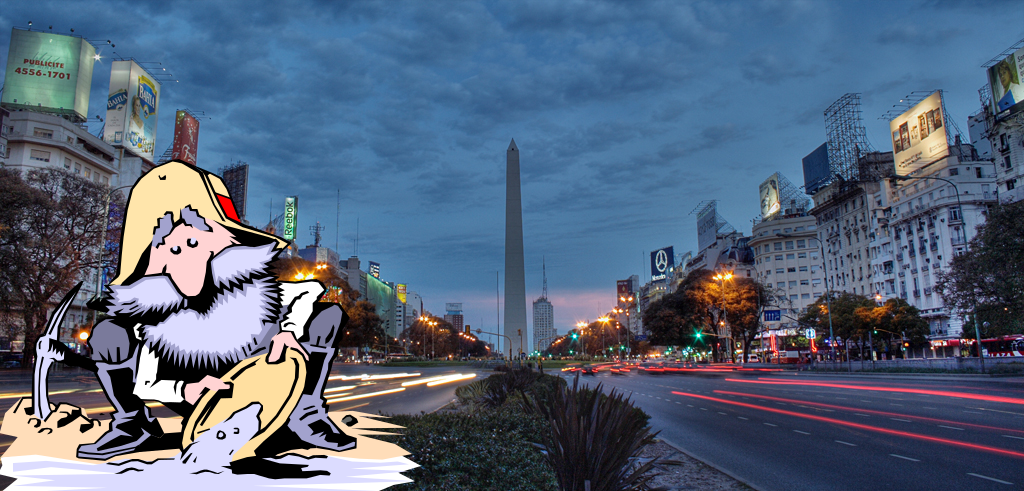
\includegraphics[width=\paperwidth,height=\paperheight]{figs/obelisco-miner.png}}

\begin{frame}

  {\bf
  
    \begin{center}
      {\Huge \textcolor[rgb]{1,1,1}{MSR 2017 in Buenos Aires!!!}}
    \end{center}

    \vspace{4cm}
    
    ~
  }
\end{frame}

\usebackgroundtemplate{}

%%-----------------------------------------------------
\begin{frame}
\frametitle{Buenos Aires}

\begin{columns}[T]
\begin{column}{.50\textwidth}
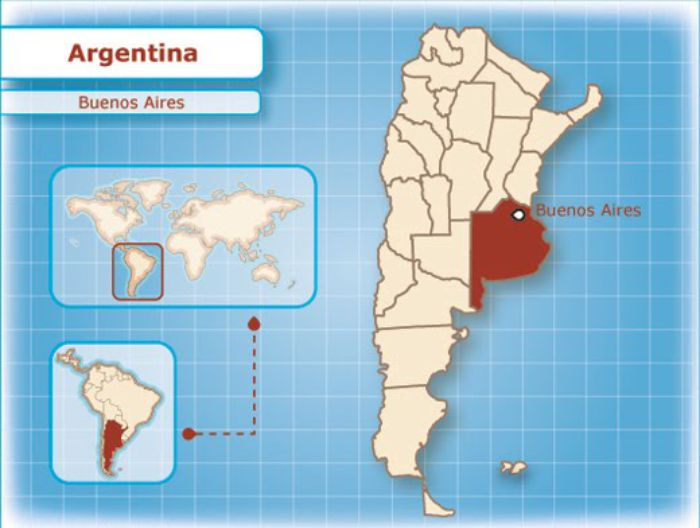
\includegraphics[width=6.5cm]{figs/argentina-in-maps}

\end{column}%
\hfill%
\begin{column}{.48\textwidth}
{\Large
\begin{itemize}
\item First time ever South of Rio Grande
\item Good opportunity for learning tango!
\item ...and for joining the MSR community
\end{itemize}
}
\end{column}%
\end{columns}

\end{frame}


%%-----------------------------------------------------
\begin{frame}
\frametitle{MSR 2017}

\begin{columns}[T]
\begin{column}{.50\textwidth}

\includegraphics[width=6.5cm]{figs/msr-miner}

\begin{flushright}
  \url{http://icse2017.gatech.edu} \\
  \url{http://2017.msrconf.org} \\
  (Coming soon!)
\end{flushright}

\end{column}%
\hfill%
\begin{column}{.48\textwidth}
{\Large
\begin{itemize}
\item Co-located with ICSE
\item Program chairs: \\
  Abram Hindle \\
  Lin Tan \\
\item General chair: \\
  Jesus M. Gonzalez-Barahona \\
%\item Venue: Universidad Católica de Argentina
\item Save the dates: \\
  May 20-21 2017 \\
\item Start the conversation!!! \\
  \textbf{\#msr17} \\
\end{itemize}
}
\end{column}%
\end{columns}

\end{frame}


%%-----------------------------------------------------
\begin{frame}
\frametitle{Double-blind for the first time at MSR!}

{\Large
MSR 2017 research \& practice paper submissions should not reveal the identity of the authors.

\begin{itemize}
\item Leave out author names and affiliations from the submission.
\item Write in third person for citations to related work by authors: ``the prior work of XYZ'' instead of ``our prior work''.
\end{itemize}

Authors having further questions on double-blind reviewing are encouraged to contact the PC chairs \\

}

\end{frame}


%%-----------------------------------------------------
\begin{frame}
\frametitle{Dates for research \& practice track}

{\Huge
\begin{itemize}
\item Abstract Deadline: \\ Feb 3, 2017
\item Full Paper Deadline: \\  Feb 10, 2017
\item Notification: \\ Mar 15, 2017
\end{itemize}
}
\end{frame}


%%-----------------------------------------------------
\begin{frame}
\frametitle{Open Mining Challenge Proposals}

{\Large
\begin{itemize}
\item Open call for MSR 2017 Mining Challenge
\item We’ll use easychair (like a mini workshop)
\item Submissions open soon (Due in July 2016)
\item 1 page description + appendix
\item A good candidate allows for many methods of analysis (general), yet enables 1 or more for kinds of specialization (specific)
\item Need the challenge ready before fall term begins (MSR Grad Courses)
\end{itemize}
}

\end{frame}


%%-----------------------------------------------------
\begin{frame}
\frametitle{Open Challenge Proposal}

{\Large
1 page proposal + optional appendix

\begin{enumerate}
\item What is your dataset?
\item What is the size of it
\item How accessible is it?
\item How generalizable is it?
\item Does it has specialized components?
\item What kind of questions do you expectchallengers to answer?
\item Give us a small sample of the data.
\end{enumerate}
}

\end{frame}

%%-----------------------------------------------------
\begin{frame}
\frametitle{Credits}

~
\vspace{4cm}

\begin{itemize}
\item {\small Picture of the miner on the Obelisco is derived from
  ``Obelisco de Buenos Aires'', picture by Jesus Alexander Reyes Sánchez in Flickr \\
  License: Creative Commons Attribution Generic 2.0 \\}
  {\footnotesize \url{https://flic.kr/p/6T8rNY}}
  % obelisco-miner.png
\end{itemize}

\end{frame}


\end{document}
